\documentclass[12pts]{article}
\input{../../../Modele/TDStyle}
\usepackage[dvips]{graphicx}
\title{ODLU MIAGE~1~: \\
  Structures de contr\^ole
}
\date{Janvier~2005}
\correctionfalse
\begin{document}
\maketitle
%\section{Exercice divers}

%\begin{exercice}[Conversion de temp\'erature]
%  La temp\'erature se quantifie d'apr\`es diff\'erentes \'echelles~:
%  \begin{itemize}
%  \item  \textit{L'\'echelle   Celsius},  qui a   pour   rep\`eres les
%    temp\'eratures~$0$C   (glace fondante)     et~$100$C
%    (\'ebullition  de l'eau) comporte,   entre ces  deux points,~$100$
%    degr\'es Celsius.
%  \item \textit{L'\'echelle  Fahrenheit}   en   usage dans  les   pays
%    anglo-saxons utilise le mercure comme   \'etalon. La glace   fonds
%    \`a~$32$F et l'eau bout \`a~$212$F.
%  \item  \textit{L'\'echelle    absolue} comprend       toujours   des
%    temp\'eratures positives, qui sont compt\'ees en Kelvin \`a partir
%    du z\'ero absolu~($0$K=$-273$C).
%  \end{itemize} 
%  \'Etablir  les r\`egles   de  conversion entre ces  \'echelles  (par
%  exemple, K=C~$+273$).
%  \par
%  Construire  un  programme   qui   permet  la  conversion  entre  ces
%  diff\'erentes \'echelles.  Apr\`es  avoir   permit la saisie  de  la
%  temp\'erature, ce   programme  devra   tout  d'abord  demander   \`a
%  l'utilisateur  de    saisir   l'\'echelle   dans     laquelle  cette
%  temp\'erature est  exprim\'ee puis  s'enqu\'erir de  l'\'echelle dans
%  laquelle on veut faire la conversion.
%  \par
%  Enfin,  ce programme  devra  permettre gr\^ace  \`a  une   boucle de
%  recommencer cette op\'eration   autant de fois que  l'utilisateur le
%  d\'esirera.
%  \ifcorrection
%  \begin{correction}
%    \input{../../TP/Verbatim/conversiontemp.c.verb}
%  \end{correction}
%  \fi
%\end{exercice}


\section{Construction de nos fonctions d'entr\'ees-sorties}
\begin{exercice}[Les fonctions putchar et getchar]
  La fonction \verb?int putchar (int c);? prend en entr\'ee un entier
  repr\'esentant le code ASCII d'en caract\`ere et affiche ce
  caract\`ere sur la sortie standard.
  \par
  La fonction \verb?int getchar (void);? r\'ecup\`ere un caract\`ere
  dans l'entr\'ee standard et le retourne.
  \par
  L'usage de ces fonctions n\'ecessite l'ajout de la directive
  \verb?#include <stdio.h>? \`a votre code.
  \par
  Construisez un programme qui permette \`a l'utilisateur de saisir
  une lettre minuscule au clavier et affiche la majuscule
  correspondante \`a l'\'ecran (ne vous occupez pas de la gestion
  d'erreur).
  \par
  M\^eme exercice mais la lettre est suppos\'ee \^etre stock\'ee dans
  un fichier et la majuscule doit \^etre stock\'ee dans un autre
  (utilisez les redirections du shell).
\end{exercice}

\begin{exercice}[Saisie d'entier avec getchar] 
\label{exercicecounter:getchar}
Construire un programme dont la fonction principale permette de saisir
un entier stock\'e dans l'entr\'ee standard (sous forme d'une
cha\^\i{}ne de caract\`eres termin\'ee par un retour chariot) et qui
le retourne.
\ifcorrection%
\begin{correction}
\input{../../TP/Verbatim/conversionASCIIEntier.c.verb}
\end{correction}
\fi%
Stocker votre cha\^\i{}ne de caract\`eres en utilisant une commande
interne du shell.  Puis, en utilisant une variable pr\'e-d\'efinie du
shell, v\'erifiez que votre programme marche correctement (attention,
la variable shell \$? est cod\'ee non sign\'ee sur un octet).
\end{exercice}

\begin{exercice}[Affichage d'entier avec putchar] 
  Construire un programme dont la fonction principale permette
  d'afficher un entier machine stock\'e dans une variable.
  \ifcorrection
  \begin{correction}
    \input{../../TP/Verbatim/conversionEntierASCII.c.verb}
  \end{correction}
  \fi 
\end{exercice}

\section{Pretty printer}

Cet exercice est tir\'e des notes de Ph.~Marquet.

Le but de ce TP est de d\'evelopper un \textit{filtre} en langage C. On
appelle filtre un programme qui lit un texte sur l'entr\'ee standard
(stdin) et qui sort un texte sur la sortie standard (stdout), avec
\'eventuellement quelques modifications. Le plus simple des filtres est
la commande Unix cat qui lit stdin et \'ecrit le m\^eme texte sur stdout.

Le filtre d\'evelopp\'e durant ce TP est appel\'e \textit{pretty-printer}
(on nommera le fichier source pp.c et l'ex\'ecutable~pp). Il permet de
mettre en forme un fichier texte contenant un programme C. On se
limitera \`a une version simplifi\'ee qui s'occupe uniquement de
l'indentation et des commentaires.


\subsection{Sp\'ecification de la commande pp}
\paragraph{Indentation}


\`A chaque accolade ouvrante, on passera \`a la ligne suivante et on
incr\'ementera l'indentation courante (par d\'efaut, on consid\'erera
qu'une indentation vaut~$4$ blancs). \`A chaque accolade fermante, on
ira aussi \`a la ligne apr\`es avoir d\'ecr\'ement\'e l'indentation.
Tout d\'ebut effectif de ligne se fera au niveau de l'indentation
courante (attention \`a la lecture de blancs ou de tabulations
'\verb?\t?' en d\'ebut de ligne).


\paragraph{Commentaires}

On placera les commentaires en d\'ebut de ligne, au niveau de
l'indentation courante. On se limitera \`a un commentaire par ligne.
Quand une fin de ligne ('\verb?\n?') appara\^\i{}t dans un commentaire, on
fermera ce commentaire et on en ouvrira un second sur la ligne
suivante.


\paragraph{Erreur}

En cas d'erreur (commentaire non ferm\'e ou texte mal
\textit{accolad\'e}), on sortira un message d'erreur sur stderr, tout
en continuant le formatage. En fin de formatage, on pourra afficher un
message d'avertissement si les nombres d'accolades ouvrantes et
fermantes ne semblent pas correspondre. L'ex\'ecution de pp se
terminera alors sur un \'echec (EXIT\_FAILURE).

\paragraph{Attention}
\begin{itemize}
\item une accolade dans un commentaire doit \^etre ignor\'ee.
\item aucune modification ne doit \^etre faite sur une ligne commen\c{c}ant
  par une directive de cpp (\#define, \#include... ou d'autres lignes
  commen\c{c}ant par `\#').
\item aucune modification ne doit \^etre faite \`a l'int\'erieur des cha\^\i{}nes
  de caract\`eres litt\'erales ("blabla"). On pourra, dans un premier
  temps, consid\'erer qu'il n'y a pas de guillemets dans une cha\^\i{}ne
  litt\'erale.
\end{itemize}

\paragraph{Exemple}
\`A partir du fichier file.c suivant :
\begin{verbatim}
#include <stdio.h>
        /* Ce programme C ne fait pas grand chose */

void main() {
   int n;
     char c;
        
       c = getchar(); /* on lit un caractere */ /* sur stdin */

if (c==' ') { n++;putchar(c);}
     else /* sinon,
             on ne fait rien */
      { ;}
}
\end{verbatim}
la ligne de commande
\begin{verbatim}
% pp < file.c > file-i.c
\end{verbatim}
va cr\'eer un fichier file-i.c qui contiendra :
\begin{verbatim}
#include <stdio.h>
/* Ce programme C ne fait pas grand chose */

void main()
{
    int n;
    char c;

    c = getchar();
    /* on lit un caractere */
    /* sur stdin */

    if (c==' ')
    {
        n++;putchar(c);
    }
    else
    /* sinon, */
    /* on ne fait rien */
    {
        ;
    }
}
\end{verbatim}
  
\subsection{Codage d'un automate}

Pour faciliter la conception, on peut coder le programme
pretty-printer par un automate. Par exemple, l'automate utilis\'e pour
supprimer les espaces ou les tabulations en d\'ebut de chaque ligne
comporte deux \'etats et les transitions suivantes entre ces deux
\'etats~:
\begin{center}
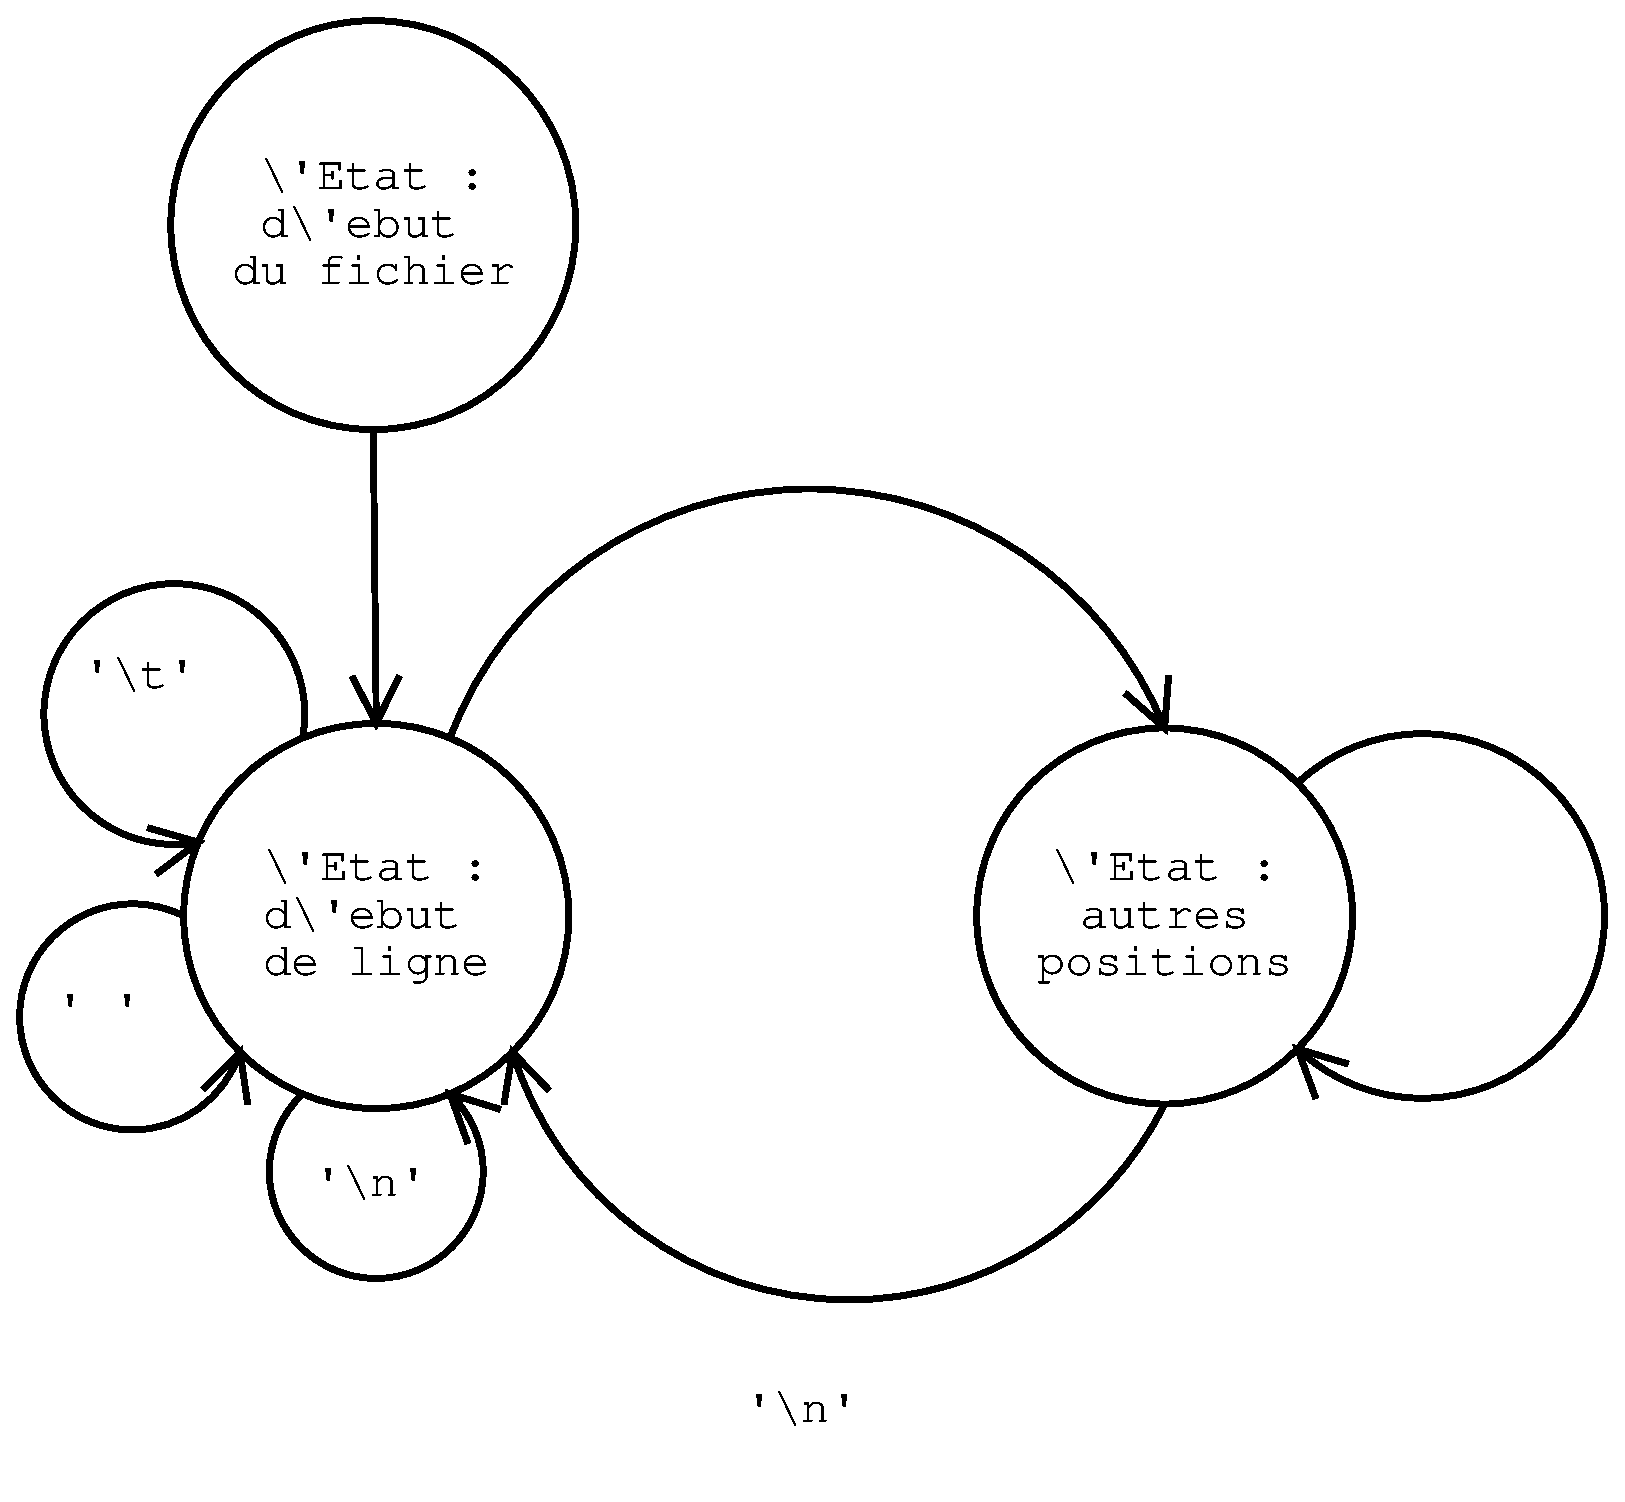
\includegraphics[scale=.3]{automatepp}  
\end{center}
\begin{exercice}[Construction d'un programme \`a partir d'un automate]
  Inspirez vous de cet automate pour \'ecrire un filtre qui supprime
  les espaces ou les tabulations en d\'ebut de chaque ligne.
   \ifcorrection%
   \begin{correction}
\begin{verbatim}
     #include <stdio.h>
#include <stdlib.h>

int 
main()
{
    int c;
    enum {ETAT_DBT_LIGNE, ETAT_NORMAL } etat = ETAT_DBT_LIGNE;
  
    while ((c=getchar()) != EOF) {
        switch (etat) {
            case ETAT_DBT_LIGNE:
                switch (c) {
                    case ' ':
                    case '\t':
                        break;
                    default:   
                        putchar(c);
                        etat = ETAT_NORMAL;
                        break;
                }
                break;
            case ETAT_NORMAL:
                switch (c) {
                    case '\n': 
                        putchar('\n');
                        etat=ETAT_DBT_LIGNE;
                        break;
                    default :  
                        putchar(c);
                        break;
                }
        }
    }

    exit(EXIT_SUCCESS);
}
\end{verbatim}
   \end{correction}
   \fi%
\end{exercice}

\subsection{Le travail restant \`a faire}
Construisez l'automate codant nos r\`egles de styles et implantez le.
\end{document}


\begin{exercice}[]
   \ifcorrection%
   \begin{correction} 
   \end{correction}
   \fi%
\end{exercice}
